\section{Experiments}
\label{sec:experiments}

\subsection{Benchmark Setup}

The benchmark plant contains three large chillers and one small chiller, a single chilled-water storage tank, normalized chilled-water and condenser-water pumping loads, and cooling-tower auxiliary power. The scheduling horizon is 24 hours with hourly resolution. The cooling load is constructed semi-synthetically from three components: a base internal load, an ambient-sensitive component, and a process-variation component. Electricity tariffs follow a time-of-use structure with higher prices during afternoon and evening hours.

We compare five benchmark methods:
\begin{enumerate}[leftmargin=1.5em]
    \item \textbf{Rule-based}: a heuristic merit-order sequencing policy with simple tariff-triggered storage charging and discharging.
    \item \textbf{Deterministic MILP without storage}: nominal day-ahead optimization with auxiliary-equipment modeling but no robustness terms and no storage use.
    \item \textbf{Deterministic MILP with storage}: nominal day-ahead optimization that isolates the value of storage without robustness.
    \item \textbf{Robust MILP without storage}: robust day-ahead optimization with uncertainty budgets for load and tariff but without storage.
    \item \textbf{Robust MILP with storage}: the full proposed formulation.
\end{enumerate}

To evaluate robustness, we additionally generate out-of-sample perturbations by sampling each load component and tariff within its bounded uncertainty interval. We report the resulting mean cooling shortfall, upper-tail shortfall statistics, and realized energy cost under the fixed day-ahead schedule. We also evaluate a correlated-stress setting in which the ambient-sensitive component receives a common adverse disturbance across the day.

\subsection{Main Comparative Results}

Table~\ref{tab:main_results} summarizes the benchmark. The deterministic MILPs deliver the lowest nominal operating cost, with the storage-enabled deterministic schedule achieving the best nominal objective at 5584.7. However, both deterministic schedules perform poorly under uncertainty, with an out-of-sample mean shortfall of 740.3~kWh. By contrast, the robust formulations sharply reduce this shortage to 66.5~kWh. Storage then recovers part of the cost premium: the robust-with-storage model lowers total cost from 6128.2 to 6002.1 relative to robust-no-storage while preserving the same shortage metric.

\begin{table}[H]
\centering
\caption{Main benchmark results.}
\label{tab:main_results}
\begin{tabular}{lrrrrr}
\toprule
Method & Total cost & Peak power & Avg. COP & OOS shortage & Energy cost \\
\midrule
Rule-based & 7230.2 & 422.1 & 2.655 & 355.7 & 7116.9 \\
Deterministic no storage & 5706.4 & 320.4 & 3.296 & 737.4 & 5628.4 \\
Deterministic with storage & 5584.7 & 341.9 & 3.279 & 740.3 & 5488.6 \\
Robust no storage & 6128.2 & 335.9 & 3.290 & 66.5 & 5852.9 \\
Robust with storage & 6002.1 & 343.8 & 3.277 & 66.5 & 5725.4 \\
\bottomrule
\end{tabular}
\end{table}

Figure~\ref{fig:dispatch} shows the 24-hour dispatch comparison. The rule-based method relies on more aggressive heuristic operation and exhibits visibly larger load-following overhead. The deterministic MILP concentrates on nominal cost minimization, whereas the robust variants allocate more cooling margin during uncertain hours. Storage smooths this behavior by shifting cooling production away from the most expensive periods.

\begin{figure}[H]
    \centering
    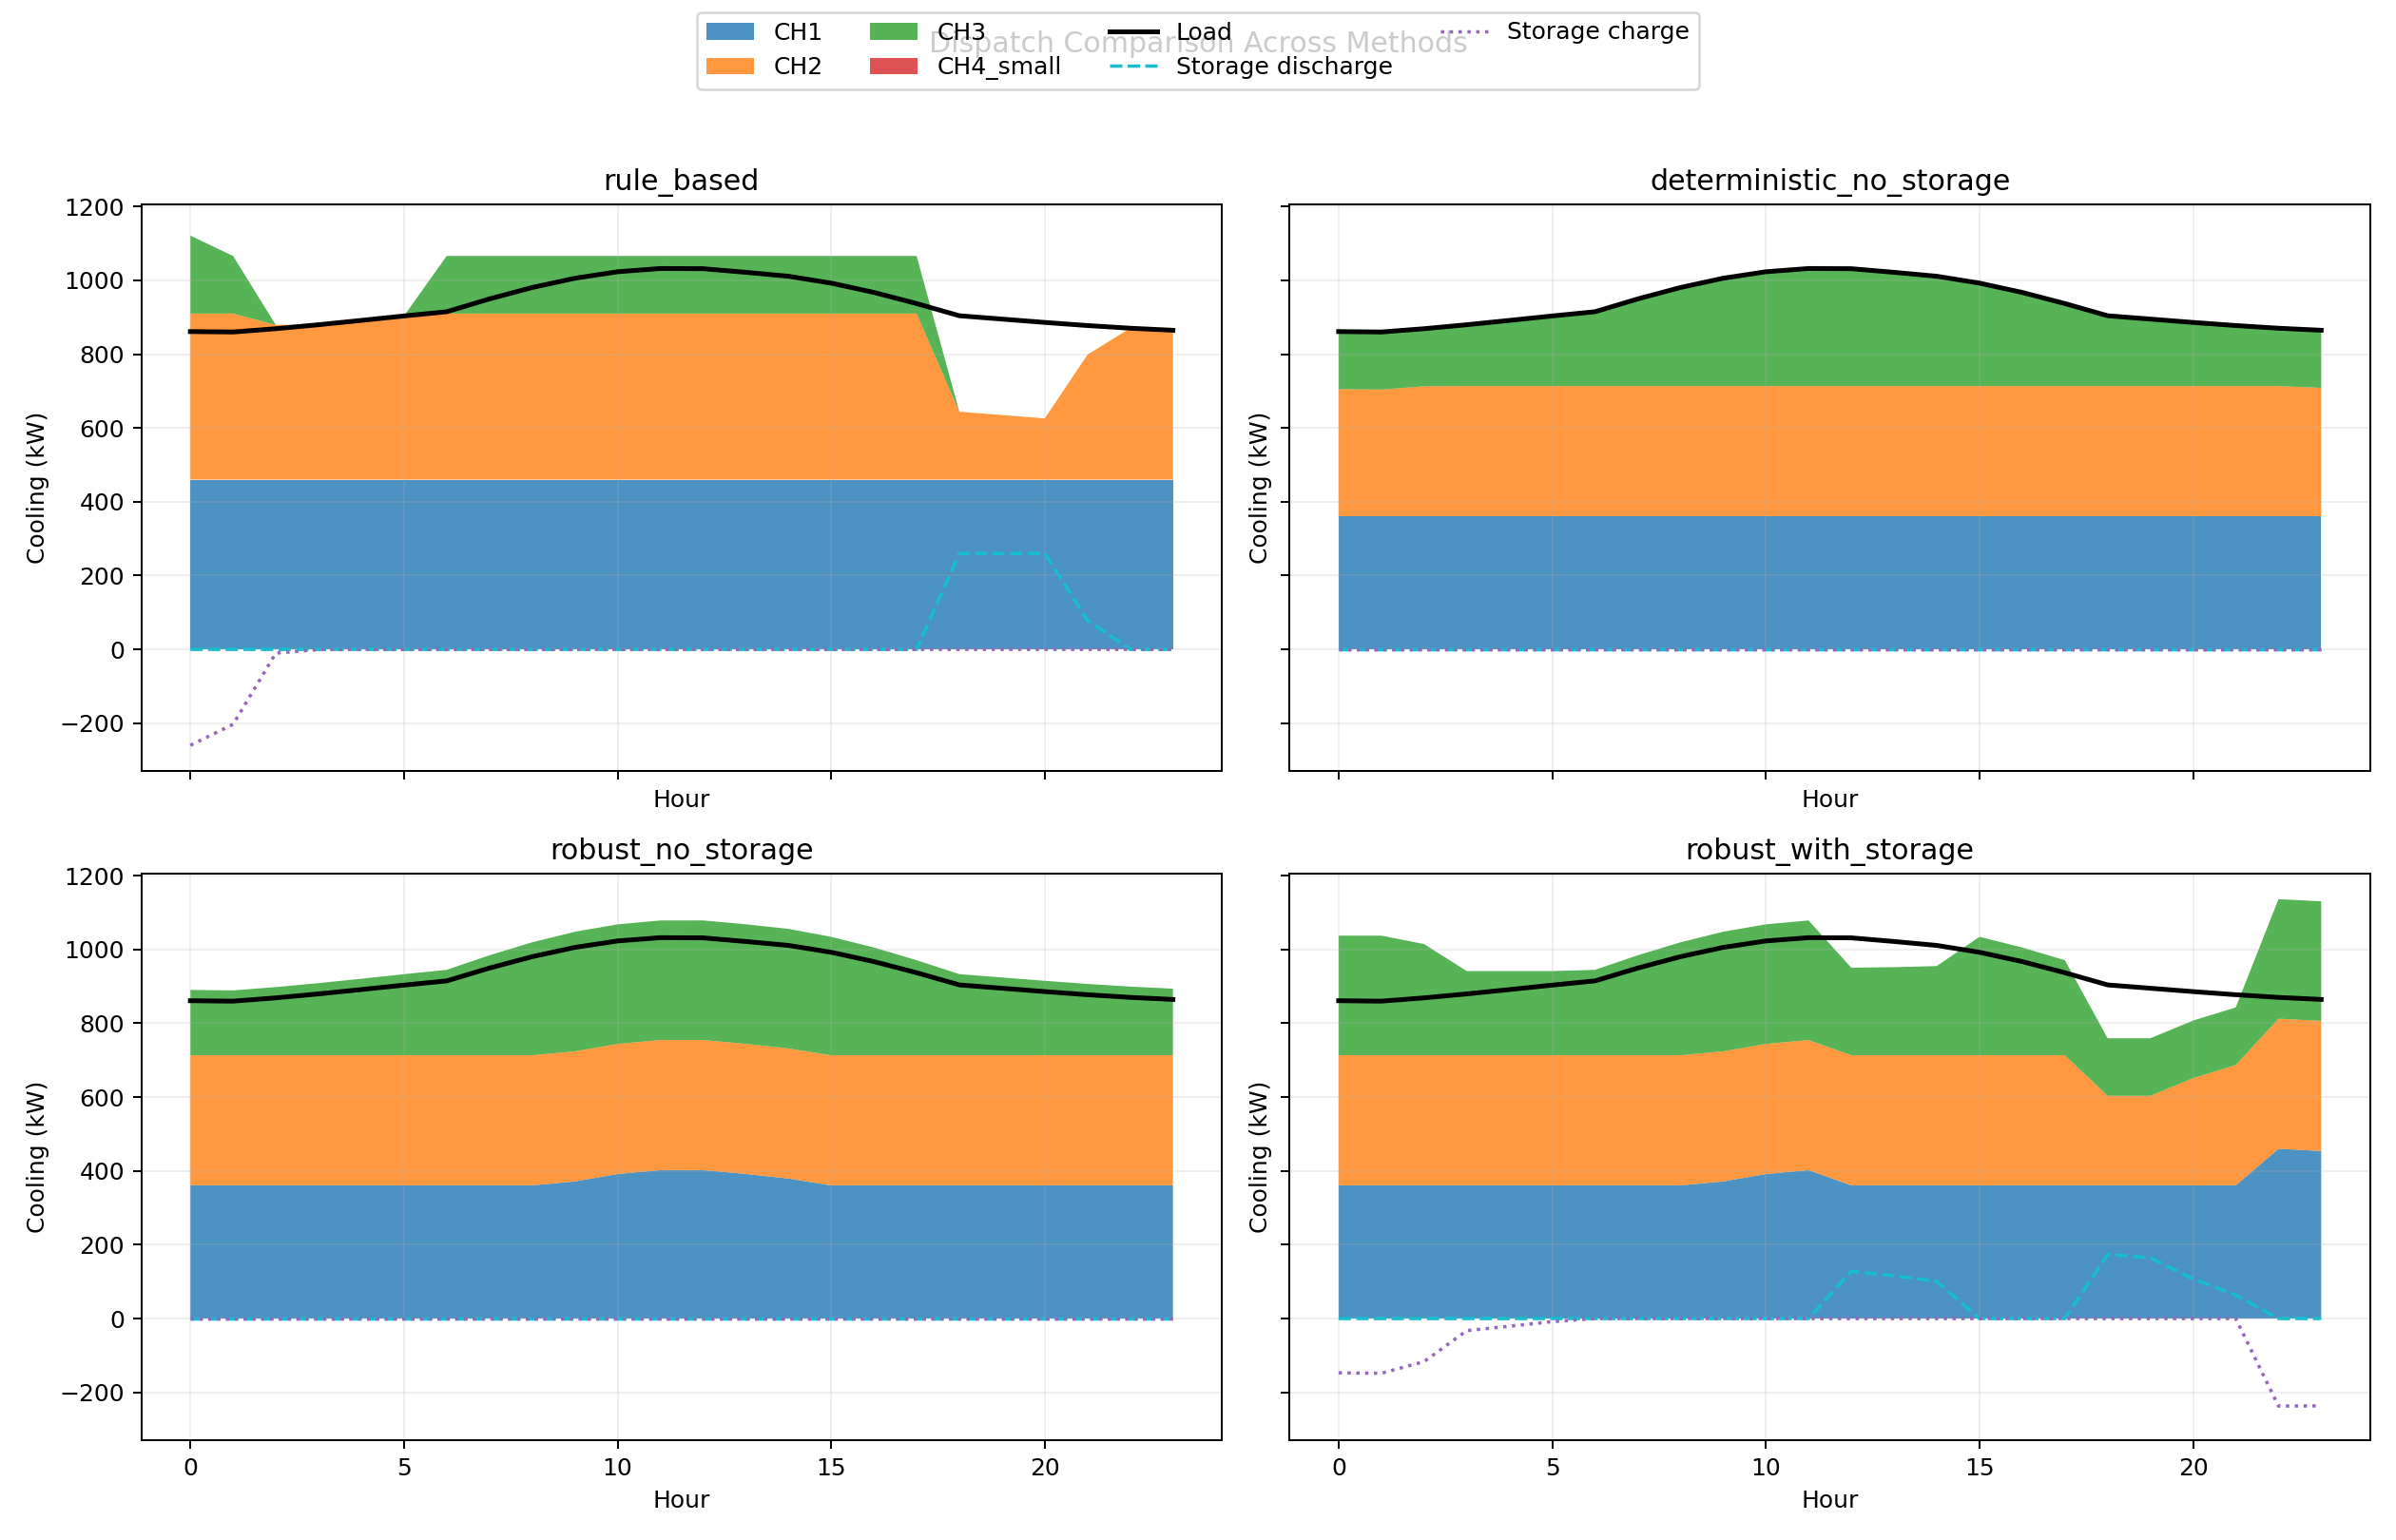
\includegraphics[width=\linewidth]{figures/dispatch_comparison.png}
    \caption{Dispatch comparison across benchmark methods. Stacked areas show chiller cooling contributions, while the overlaid load and storage traces highlight day-ahead load shifting.}
    \label{fig:dispatch}
\end{figure}

Figure~\ref{fig:tradeoff} makes the key tradeoff explicit. Moving from the deterministic MILP to the robust MILP requires a modest increase in total cost, but it substantially improves out-of-sample cooling adequacy. This behavior is desirable for operators that face penalties or service risks from under-delivered cooling.

\begin{figure}[H]
    \centering
    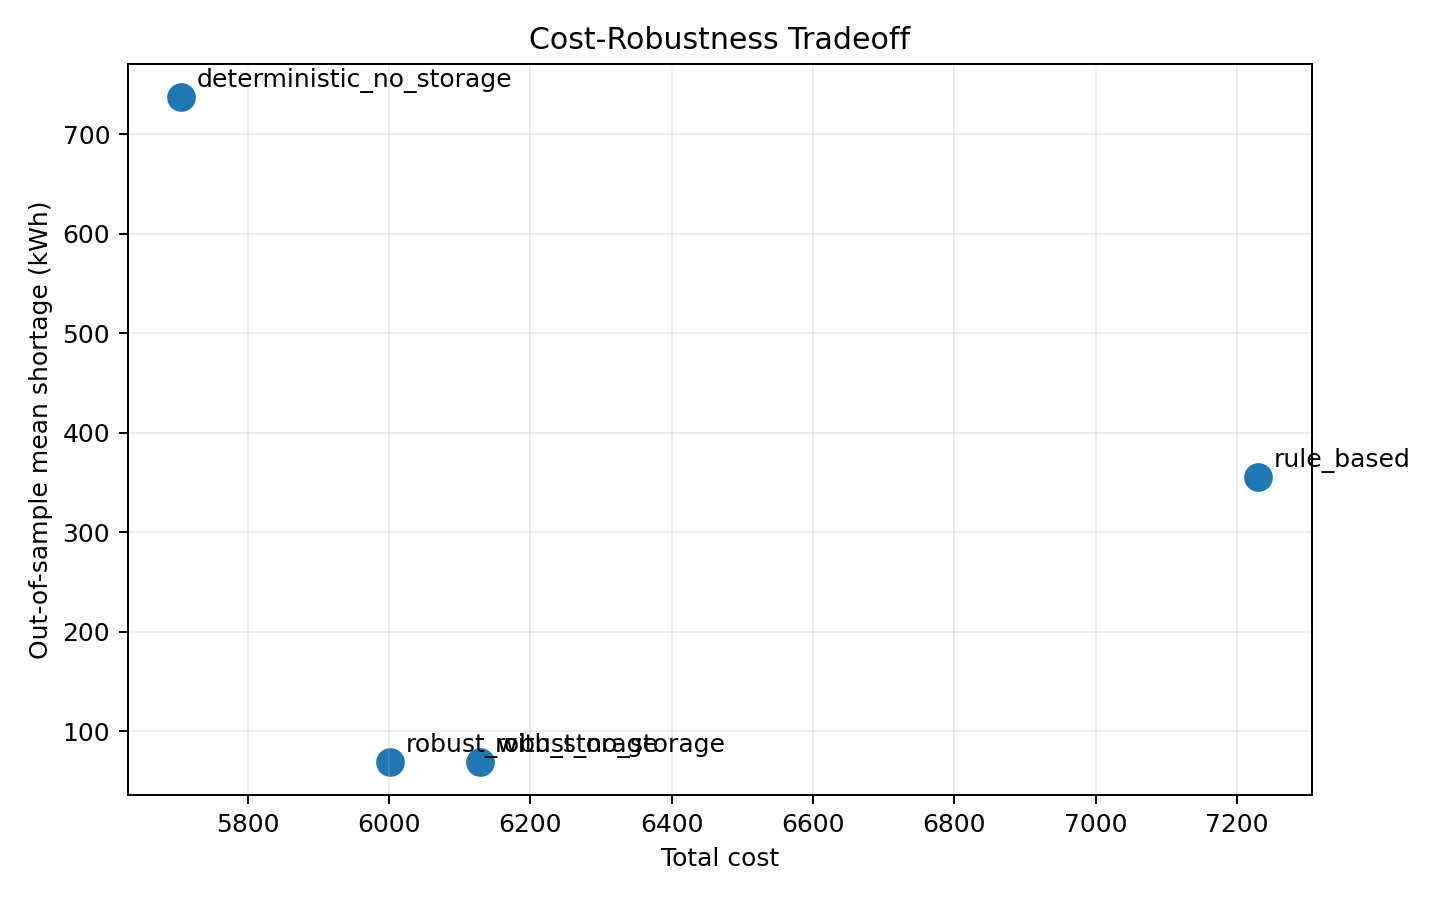
\includegraphics[width=0.74\linewidth]{figures/cost_robustness_tradeoff.png}
    \caption{Total-cost versus out-of-sample-shortage tradeoff for the benchmark methods.}
    \label{fig:tradeoff}
\end{figure}

\subsection{Storage and Auxiliary-Equipment Interpretation}

The robust-with-storage solution does not minimize peak grid power in this benchmark, because it opportunistically charges during lower-price hours to protect future adequacy. This is visible in Figure~\ref{fig:grid_soc}, where state-of-charge trajectories differ markedly across methods. The value of storage here is therefore not merely peak shaving; it also acts as a flexibility buffer that lowers total cost under robust planning constraints.

\begin{figure}[H]
    \centering
    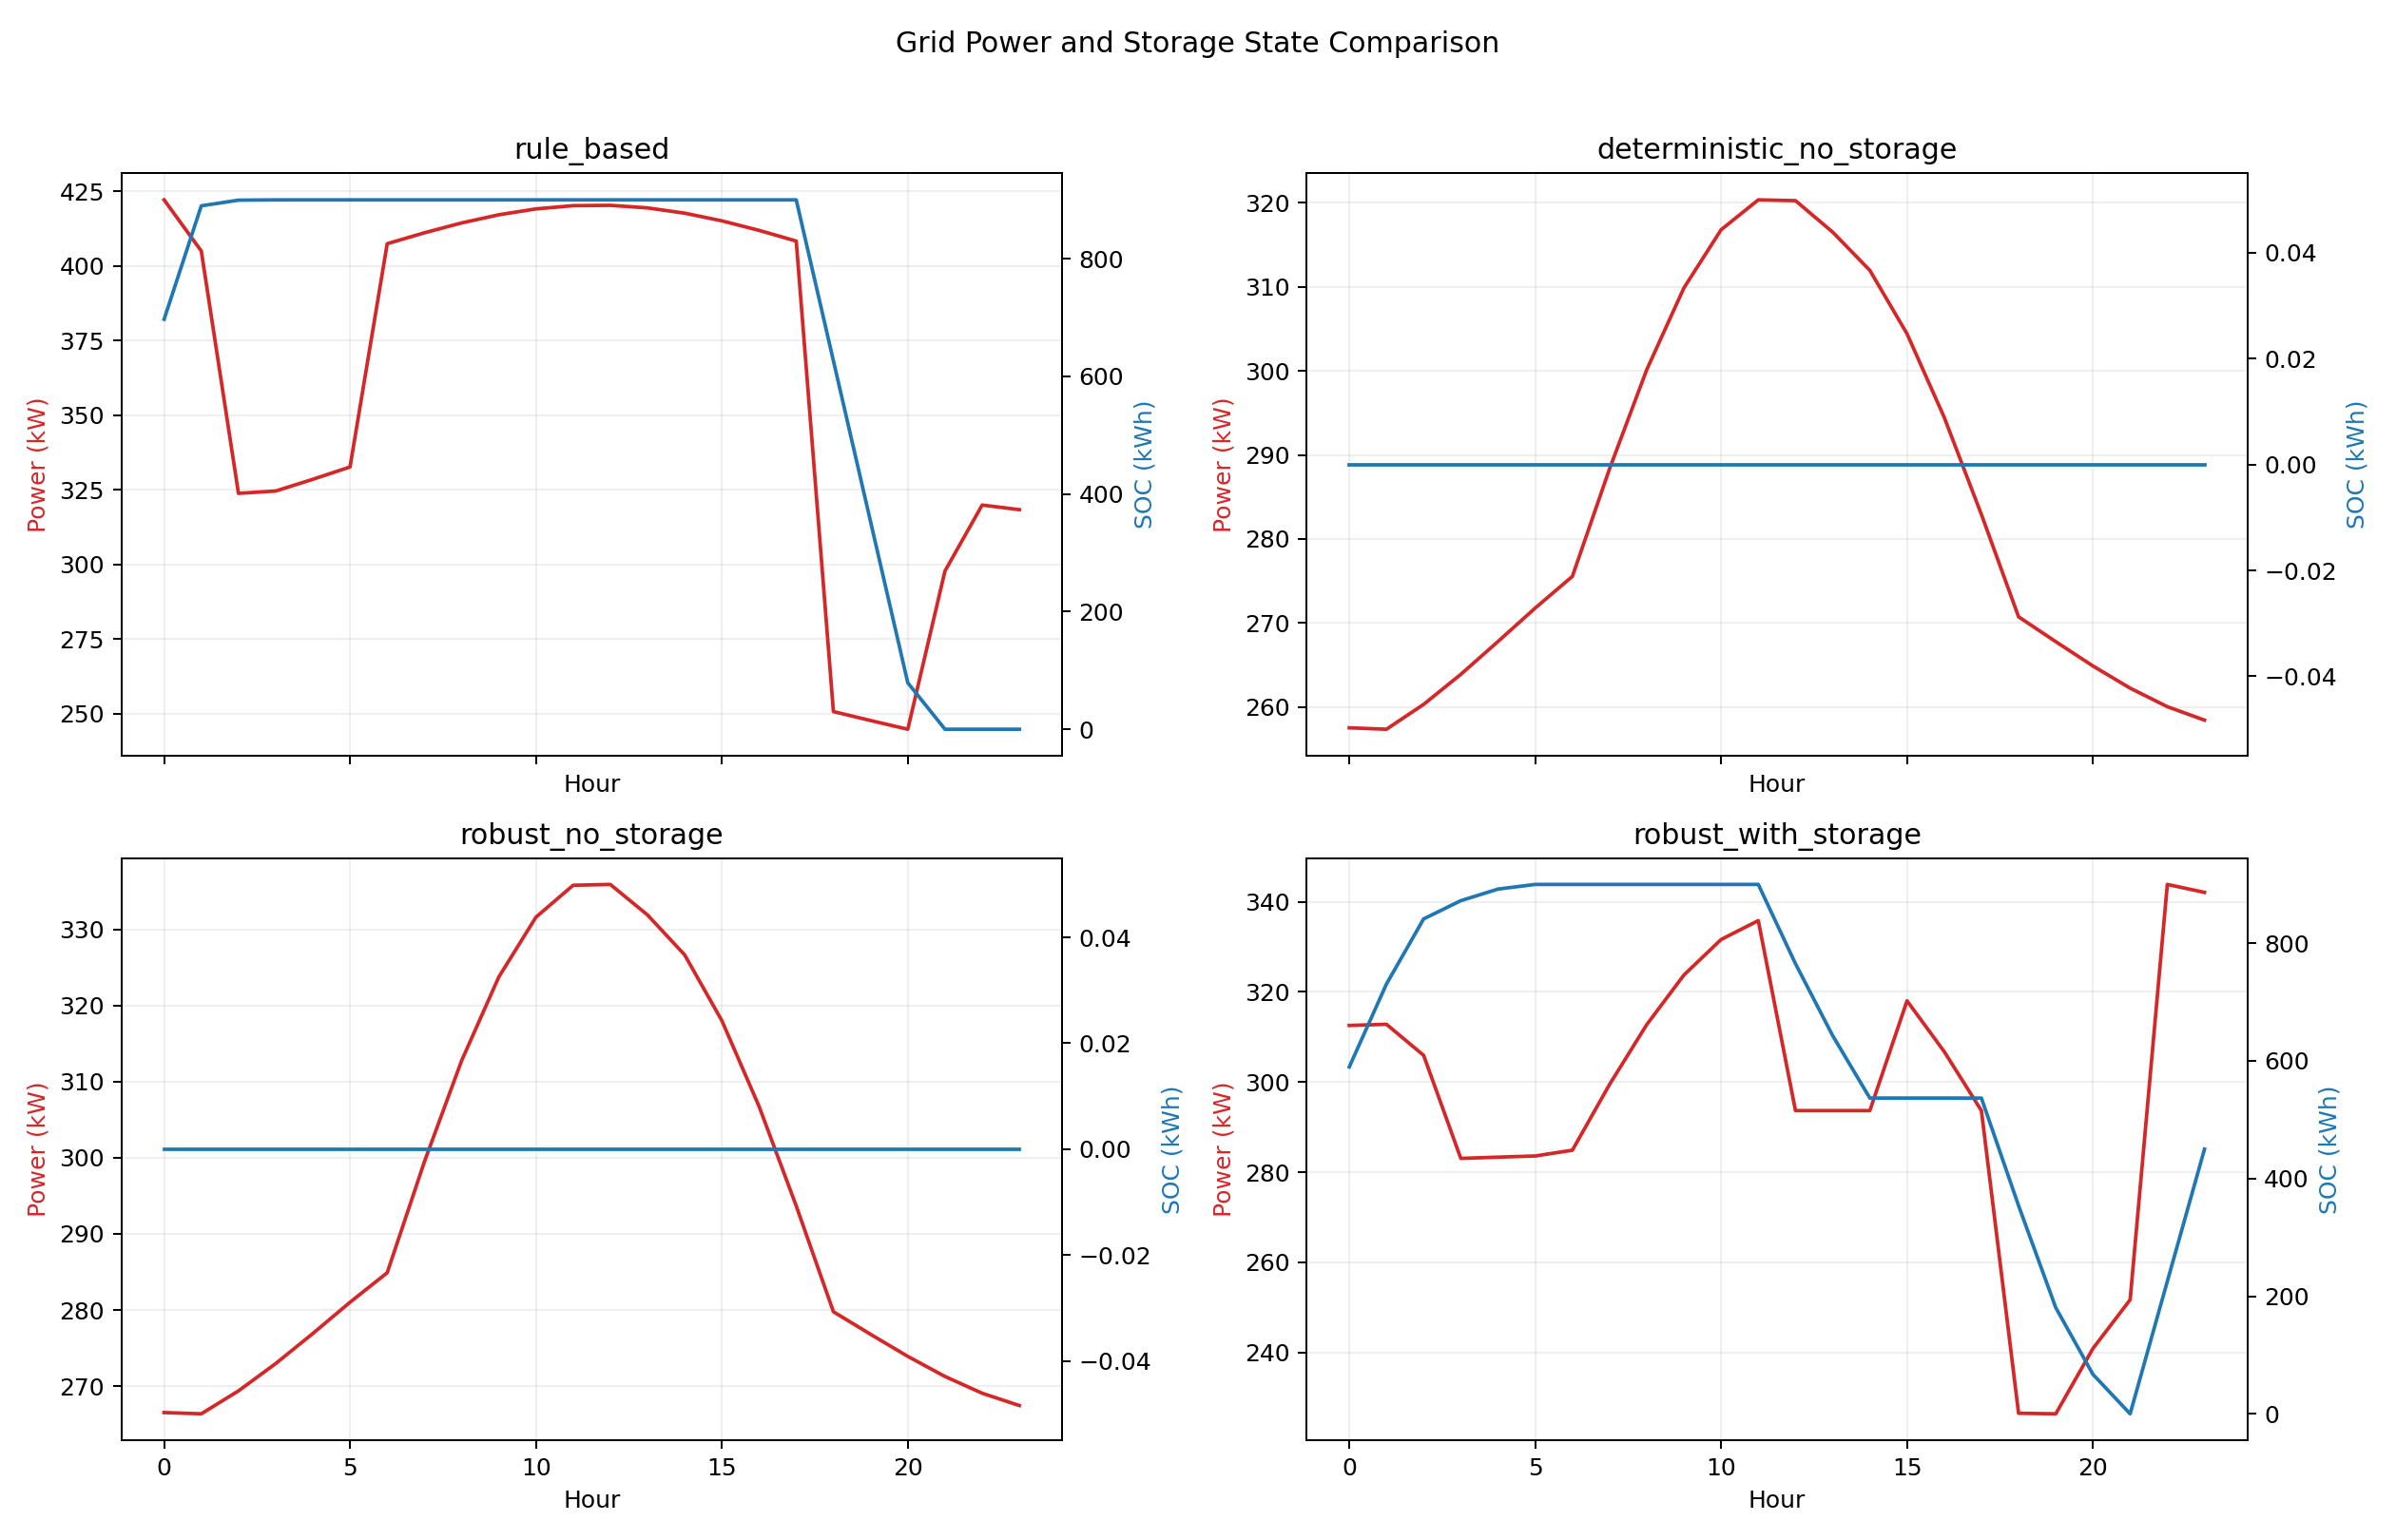
\includegraphics[width=\linewidth]{figures/grid_soc_comparison.png}
    \caption{Grid power and storage-state comparison. Storage changes when cooling is produced rather than simply reducing the instantaneous peak at all times.}
    \label{fig:grid_soc}
\end{figure}

The cost decomposition in Figure~\ref{fig:cost_breakdown} further clarifies the mechanism. Relative to the rule-based baseline, optimization reduces nominal energy cost substantially. Relative to deterministic scheduling, robust scheduling introduces a tariff-risk premium and more conservative dispatch decisions, but these are partially offset by storage-enabled temporal shifting. The robustness benefit is not limited to the mean: the deterministic schedules have a 95th-percentile shortfall of approximately 802.2~kWh, whereas the robust schedules reduce that value to 98.2~kWh. Under the correlated-stress evaluation, the mean shortage drops from 528.0~kWh for deterministic-with-storage to 23.0~kWh for robust-with-storage.

\begin{figure}[H]
    \centering
    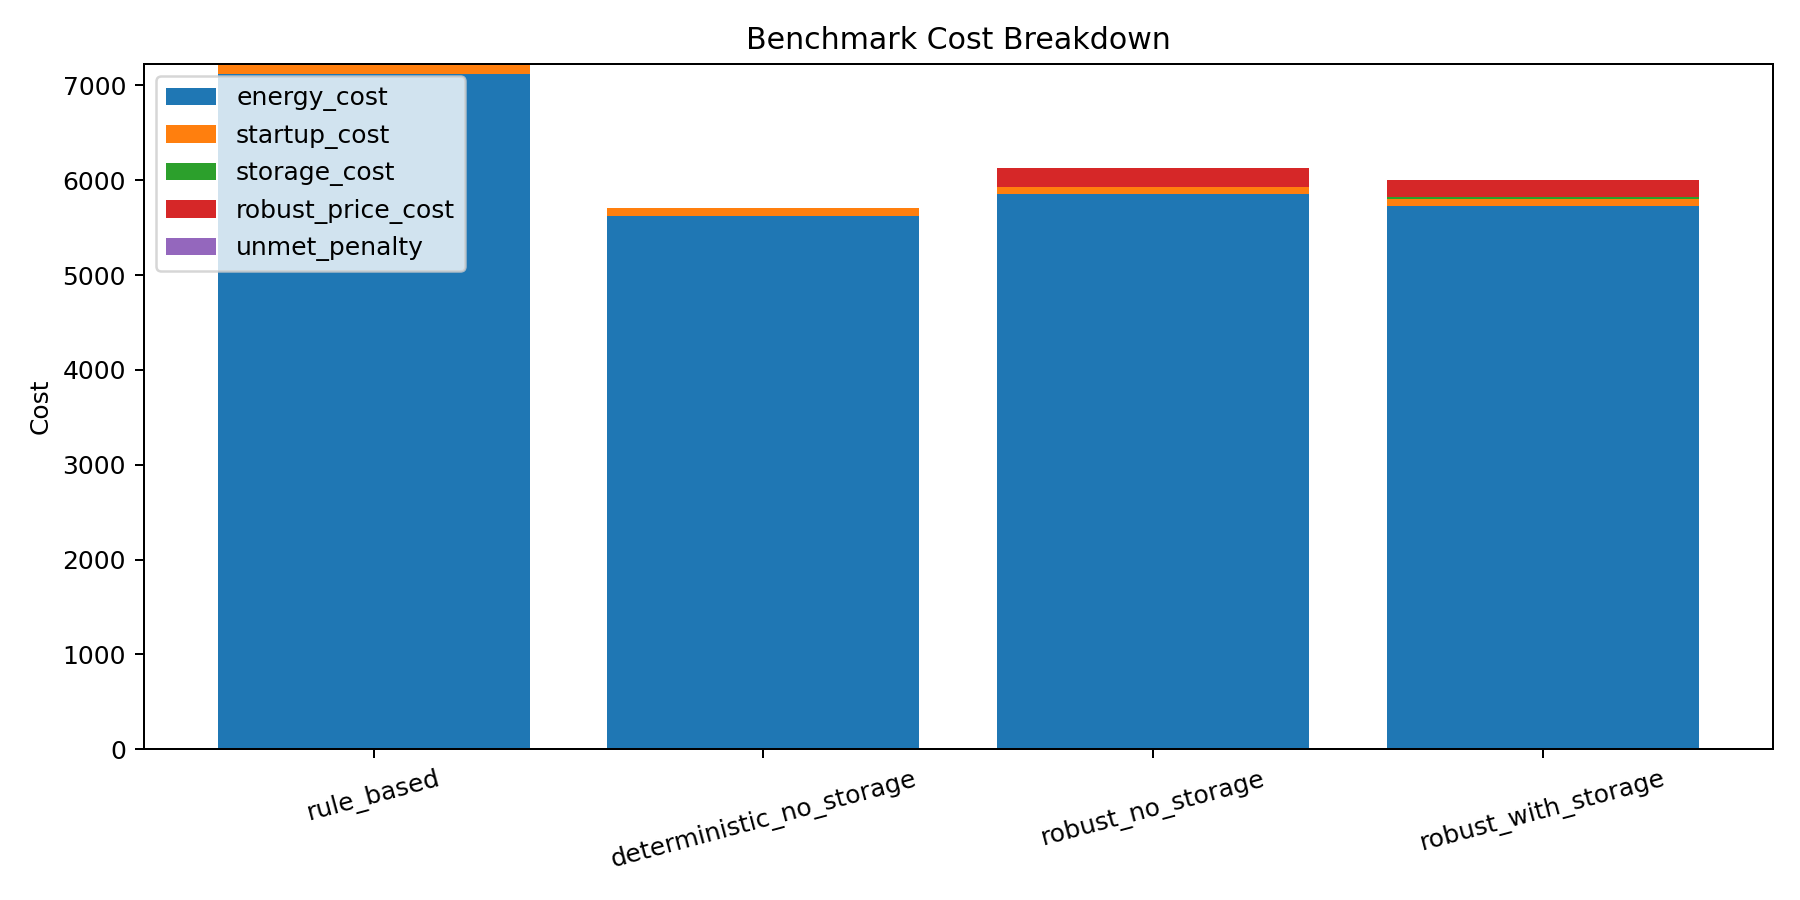
\includegraphics[width=0.84\linewidth]{figures/cost_breakdown.png}
    \caption{Benchmark cost breakdown by method.}
    \label{fig:cost_breakdown}
\end{figure}

\subsection{Ablation Studies}

We next examine how the robustness budget $\GammaL$ affects performance. As shown in Figure~\ref{fig:gamma}, increasing $\GammaL$ from 0.0 to 2.2 raises total cost from 5584.7 to 6092.8, but it drives the out-of-sample mean shortage down from 737.4~kWh to 2.8~kWh. This monotonic trend indicates that the uncertainty-budget parameter is interpretable and operationally tunable.

\begin{figure}[H]
    \centering
    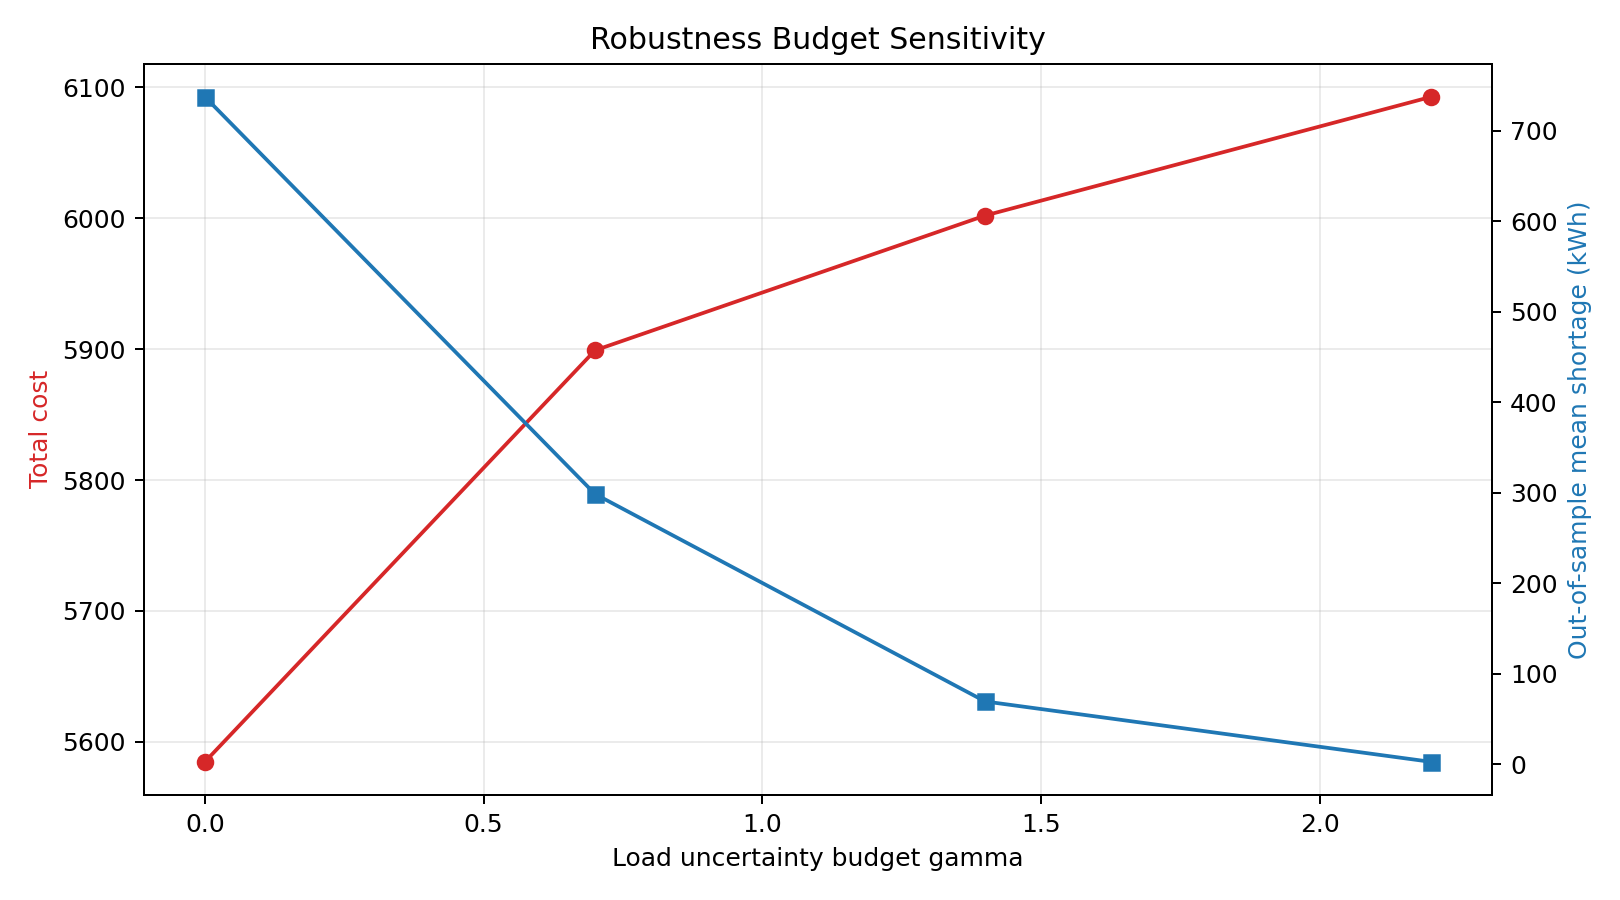
\includegraphics[width=0.78\linewidth]{figures/gamma_sensitivity.png}
    \caption{Sensitivity to the load uncertainty budget. Larger budgets increase cost but significantly reduce out-of-sample shortage.}
    \label{fig:gamma}
\end{figure}

Storage sizing yields a different pattern. Increasing storage capacity from 450~kWh to 1400~kWh reduces total cost from 6062.0 to 5955.2, while slightly lowering the equivalent cycling ratio. This suggests that larger storage improves dispatch flexibility before cycling saturation becomes a dominant constraint.

\begin{figure}[H]
    \centering
    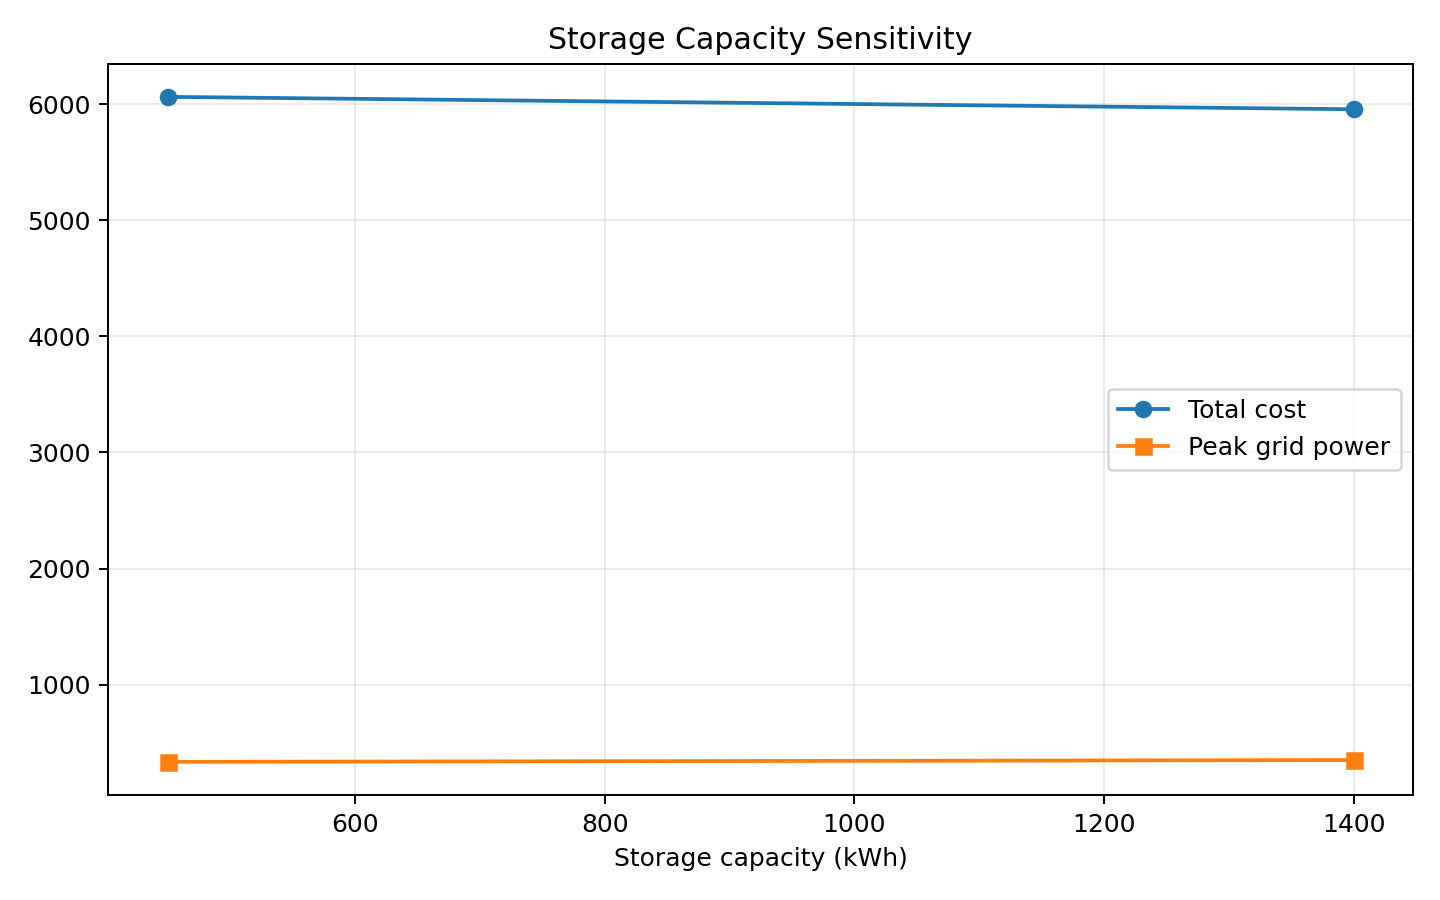
\includegraphics[width=0.74\linewidth]{figures/storage_sensitivity.png}
    \caption{Storage-capacity sensitivity. Larger storage improves total cost in the current benchmark.}
    \label{fig:storage}
\end{figure}

Two additional ablations are also informative. First, forcing identical chiller efficiency assumptions degrades average COP and increases total cost, indicating that equipment heterogeneity is not a cosmetic modeling detail. Second, removing pump and tower power terms makes the plant appear artificially efficient. This confirms that a meaningful plant-level scheduling benchmark should include auxiliary electricity use even in a simplified MILP. For completeness, the optimization runs quickly in this benchmark: solve times are around 0.09--0.13~s on the current machine, consistent with the model being intended for planning-oriented use.

\subsection{Discussion}

The results support three conclusions. First, deterministic plant scheduling can be misleadingly optimistic when the control objective includes reliable cooling adequacy under uncertainty. Second, storage has planning value beyond straightforward arbitrage because it gives the robust scheduler another degree of freedom for adequacy preservation. Third, a compact robust MILP can already produce interpretable tradeoffs and broad ablations in a fully reproducible workflow, even before field-calibrated dynamics are introduced.

At the same time, this study is intentionally limited. The benchmark is semi-synthetic rather than calibrated to field data, the uncertainty set is interval-based rather than distributionally robust, and the model uses affine auxiliary-equipment surrogates instead of detailed hydraulics. The comparison set also does not yet include a scenario-based stochastic scheduler, so the current evidence should be interpreted as a benchmark study rather than a definitive ranking across all uncertainty-aware methods.
